\chapter{Introduction}
\label{chp:introduction}
%  \citep{}
In recent years, multimedia content contributes to most of the Internet traffic and the weight is
continuously increasing. It is estimated that video traffic will be 82 percent of all consumer traffic by 2021,
up from 73 percent in 2016 \citep{vniciso}. Traditionally, video service is relied on the cloud server,
especially on "Content Distribution Nerwork"(CDN). The video providers have to pay more and more money to purchase
more resource from CDN providers to meet the exponentially growing video demand, which is not
cost-effective. Due to the huge network traffic resource used for video service, any new paradigm that
can cut down the cost and offload such demand would have a huge impact.

As many nowadays so-called lightweight device that connect to the Internet have
 better bandwidth,storage and computation capacities(such as Wi-Fi routers,Network
Attached Storage,Smart home center,etc.), these devices have the ability to provide many
types of service which can only offered by the cloud server in the past. Therefore, a new computing paradigm
based on these devices emerges with various names, such as edge computing \citep{edgecomputing},
crowdsourcing computing \citep{Chen2015Thunder} and fog computing. Fog devices also have many nicknames,
such as nano/nano data centers \citep{Valancius2009Greening} and edge device \citep{Laoutaris2008ECHOS}.
Despite the various names,the key philosophy is to use lightweight(but already powerful enough) and
close-to-user device to serve the users with lower cost and better responsiveness. In this thesis,
we use fog computing to represent all such related terms.
Our work focuse on fog-based video distribution and access. Though fog-based content distribution
and access is promising for video service, it faces challenges that have not been addressed by the
previous work on P2P paradigm or colud-based CDN.

\section{Video Popularity Characteristics}
 Any video distribution paradigm has to consider and utilize the video popularity characteristics,
in oder to effectively distributing video content. Various work has been sure that the distribution
of video popularity is skewed. At the same time, video popularity updated very quickly with
time. Therefore, the freshness of the video  content is also a very important factor when deciding
which content  to distribute. So that, we study both popularity and freshness property of video service
nowadays.
\subsection{Popularity}
Video popularity is skewed for both the video made by the user or professional generated content. For
the famous user generated content platform such as 	YouTube and Daum (a popular site in Korea),it is
shown that both of their video popularity patterns follow the Zipf distribution with exponents between
1.5(Daum) and 2.5(YouTube)for the popular videos \citep{Cha2009Analyzing}. In other word,by storing only 10 \% of long-term
popular videos, a cache can serve 80\% of requests \citep{Chen2017Migrating}.	Similar results are
confirmed by many works that masure the user preference \citep{edgecomputing} \citep{Chen2015Thunder} \citep{Huang2007Can}
 \citep{Ma2016Understanding}.Althrough both the user and professional generated content have the long
tail problem, the video in long tail are not fitness stored in the fog device, instead of stored in
the cold would be a better choice.

 \subsection{Freshness}
Statistics from various video service platform indicates that nearly 90\% of the most popular
videos(the top 10 percentile) are new videos each day. Therefore, for any video distribution system,
it has to update new contents to the fog nodes in time. Also it is  difficult to predict the popularity
of a new "User Generated Content"(UGC),which is quite the contrary in the professional generated content
by the big data and "Artificial Intelligence"(AI) approaching. As the end user demands follow a daily
pattern. The demand pattern has 2 peaks at around 1 P.M. and 10 P.M. every day. The traffic reaches its
lowest at around 4 A.M.(see in the Figure \ref{fig_1}). It is preferred to push the new contents when the user demand reaches its daily
minimal.
\begin{figure}[htbp]
\centering
	\vskip 1.0cm
	  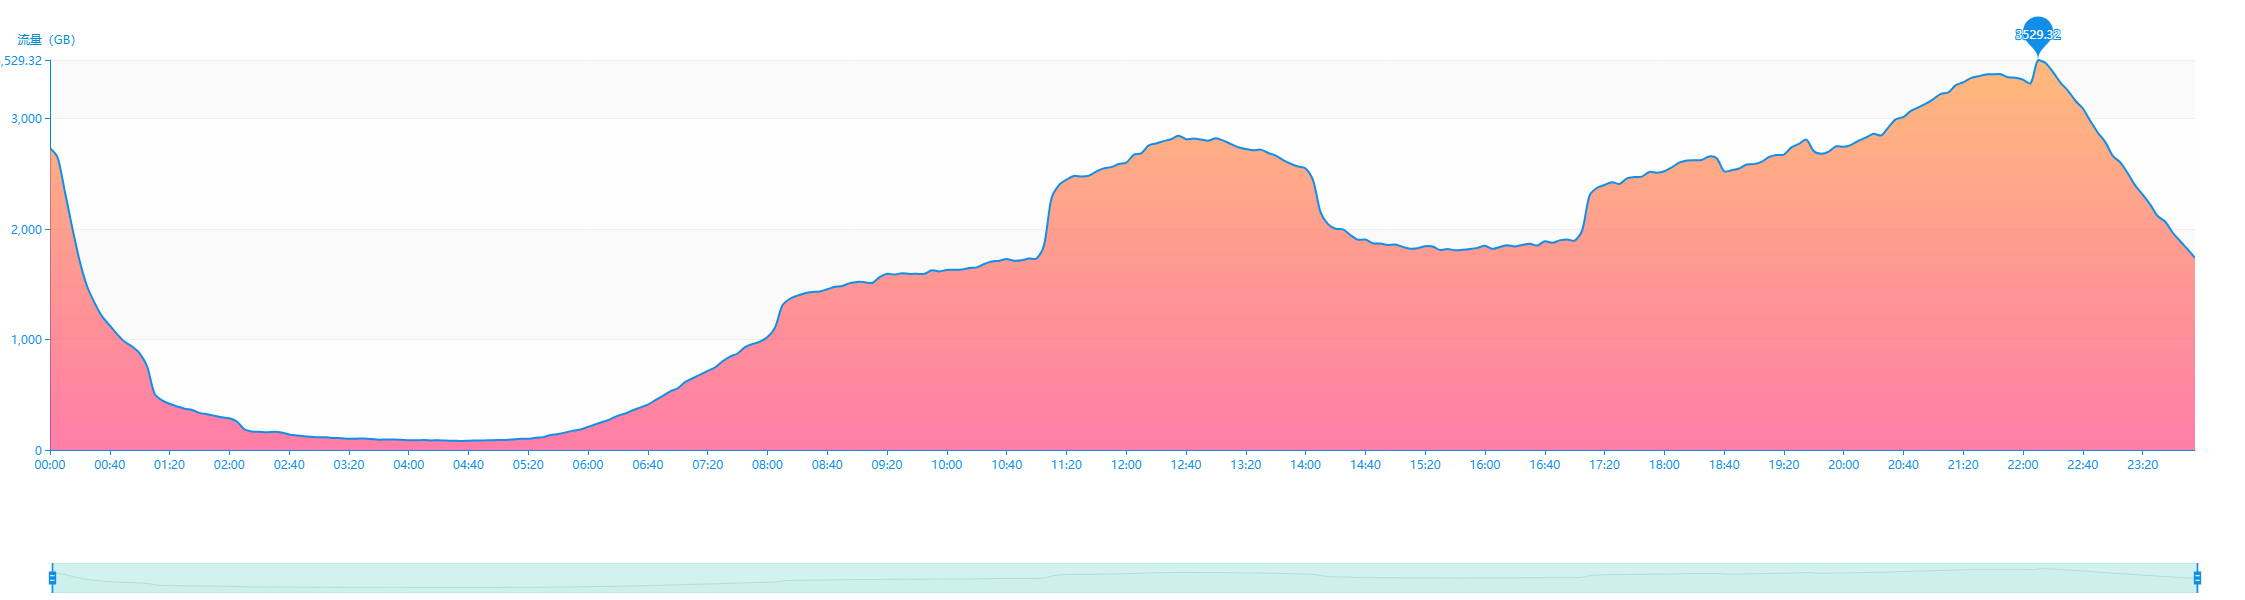
\includegraphics[width= \textwidth]{fig_1.png}
\caption{User traffic in five minutes from tencent video}
 \label{fig_1}
\end{figure}

\section{Fog Computing}
"Fog-based Concent Delivery Network"(Fog CDN), a new video delivery paradigm, which is enabled by fog nodes
(such as Wi-Fi routers,Network Attached Storage,Smart home center,etc.) deployed at users' home, becomes
the most popular topic applying in video replication and access. This  new paradigm is different from
the traditional P2P system, because it's too difficult to operating millions of dedicated
fog nodes  by the centralized video service providers in a coordinative manner\citep{Ma2016Understanding}.
Therefore, a fog-based video delivery and access network would have a huge demand gap.
\subsection{The System Architecture for CDN,P2P And peer CDN}
\begin{figure}[htbp]
\centering
	\vskip 1.0cm
	  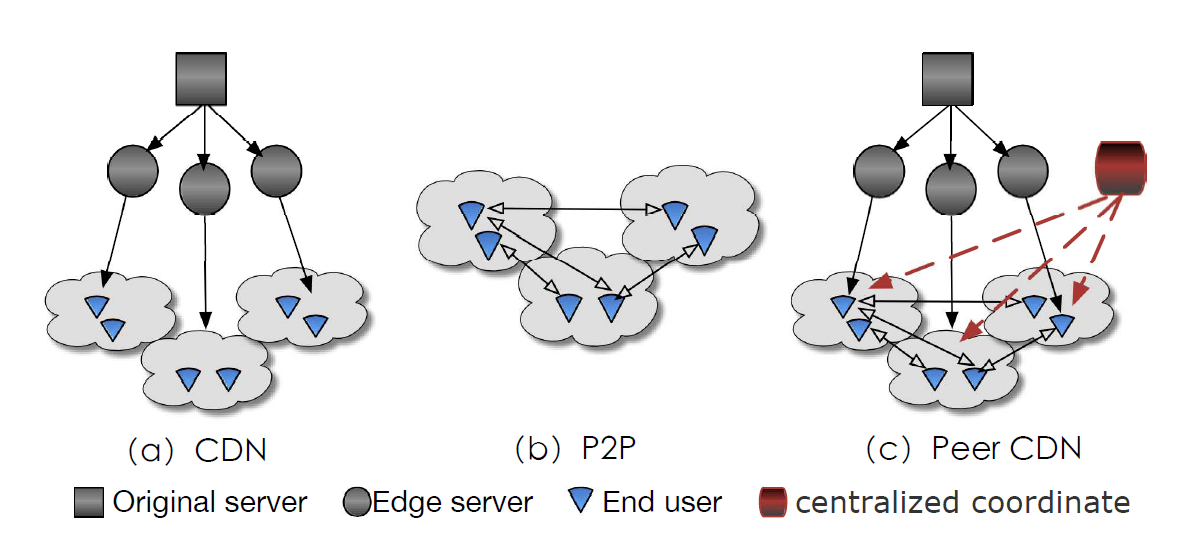
\includegraphics[width= 0.8\textwidth]{fig_2.png}
    \caption{The system architecture for CDN, P2P and peer CDN \citep{Ma2016Understanding}}
	\vskip 1.0cm
 \label{fig_2}
\end{figure}
In Figure \ref{fig_2}, it plot today's content delivery paradigms including conventional CDN,
P2P and peer CDN. Compared with the conventional CDN approach, peer
CDN employs network resources which are much closer to
users, while compared to the conventional P2P paradigm
where users individually cache and serve each other, the nodes
in a peer CDN are closely coordinated by the centralized
knowledge. For example, the content providers schedule nodes
in a peer CDN to proactively cache content, and redirect users
to download content from particular fog nodes. Today, traditional
content providers and such peer CDN providers even
start collaborating to change the traditional content delivery
paradigm, to satisfy the ever increasing generated content and
edge network requests \citep{Ma2016Understanding}.
\subsection{Fog Computing}
Research on fog computing is still in very early stages. On 19 November 2015,
ARM, Cisco, Dell, Intel, Microsoft and Princeton University formed the OpenFog Consortium.
It plans to set up seven different working groups aiming at solving problems in
fog computing, but so far it has only published one architectural white paper \citep{Cheng2014RFC}.

To integrate with the grid and interoperate with other systems, there are problems
like synchronisation and voltage control remaining to be solved. All of them require
replacement of hardware. In contrast, most fog problems lie in the software layer
and can be easily solved by complying with unified protocols. Because of the RTT-throughput
relationship(See Appendix \ref{chap:appA}) and fog’s inherent proximity to the sensors at a local environment,
 the demand for fog computing keeps growing.

\section{Development of Hardware}
In the past few years, we have witnessed the explosive growth of fog devices, as well as
their utilities and functionalities.
\subsection{IoT andWearable: Barrier and Standardisation}
In the past few years, many people have swarmed into the field of wearable devices.
However, we have also witnessed a falling of the tide. For wearables, the bottleneck is
the batteries, which require a significant breakthrough in another domain, which is not
predictable.
On 13 January 2014, Google acquired Nest for USD 3.2 billion. This acquisition triggered
a swarm into the Smart Home concept. Although people have tried IoT for many
years, Apple even emphasising it in late 1970s, the largest barrier to IoT’s market penetration
is the disunity in standard protocol adoption. Each manufacturer has used its
own proprietary protocols and technologies and has been unwilling to be connected to
(let alone controlled by) something from another vendor. The good news \citep{Bille2016RTCSS} is that we are
starting to see some moves towards standardisation.
\subsection{Smart Routers}
On 23 April 2014, XiaoMi launched an OpenWrt-based smartWi-Fi router with 1TB NAS.
It was a landmark event that motivated a lot of hardware vendors as well as Internet
software service companies to crowd into this market. Lenovo introduced NewWiFi, also
on top of OpenWrt. Huawei released Honor Router, which runs a proprietary version
of embedded Linux. Google announced OnHub, which runs Chrome OS. All the three
became “phenomenal products”. They have tried to penetrate the market with smart Wi-
Fi routers due to two main factors:
 \begin{itemize}
 	\item Wireless routers are entry points of users’ data traffic.
  \item Wireless routers are control centres in smart homes.
 \end{itemize}
However, we have now reached a turning point. "MediaTek" (MTK), the fourth largest
fabless IC designer in the world has been powering its Wi-Fi router SoCs with the ARM
Cortex architecture, which is the same as that of the CPUs used in most smartphones,
tablets and TV-boxes.

From a partner company specialising in ODM solutions for routers, we have learned
that MTK has launched a new wireless chipset product-line using the said ARM architecture.

In the Cloud, it is an access point working at the edge; in Home Entertainment, it is a
media centre; in the IoT, it is a controller of all sensors; in the Fog, it is a member of the
distributed service pool.

Briefly speaking, a fog node is a micro data centre that descends the intelligence and
resources from the core to the edge of the Internet, enabling the innovative capabilities to
provide novel and refined applications and services.

\subsection{Larger Memory and Storage at Lower Prices: A Continuous Trend}
According to the Moore's law(Figure \ref{fig_3}), the DRAM costs are dropping about 32\% every 12
months. These would be a support for bringing large buffering, caching, and storage
capacity to edge devices.

\begin{figure}[htbp]
	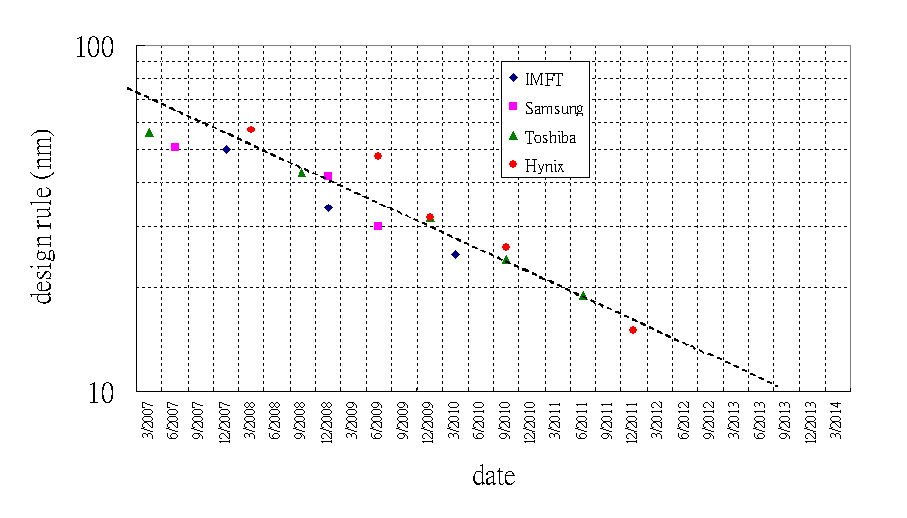
\includegraphics[width=0.8\textwidth]{fig_3}
	\caption{The trend of scaling for NAND flash memory }
	\label{fig_3}
\end{figure}
